\begin{figure}[!htb]
    \begin{center}
    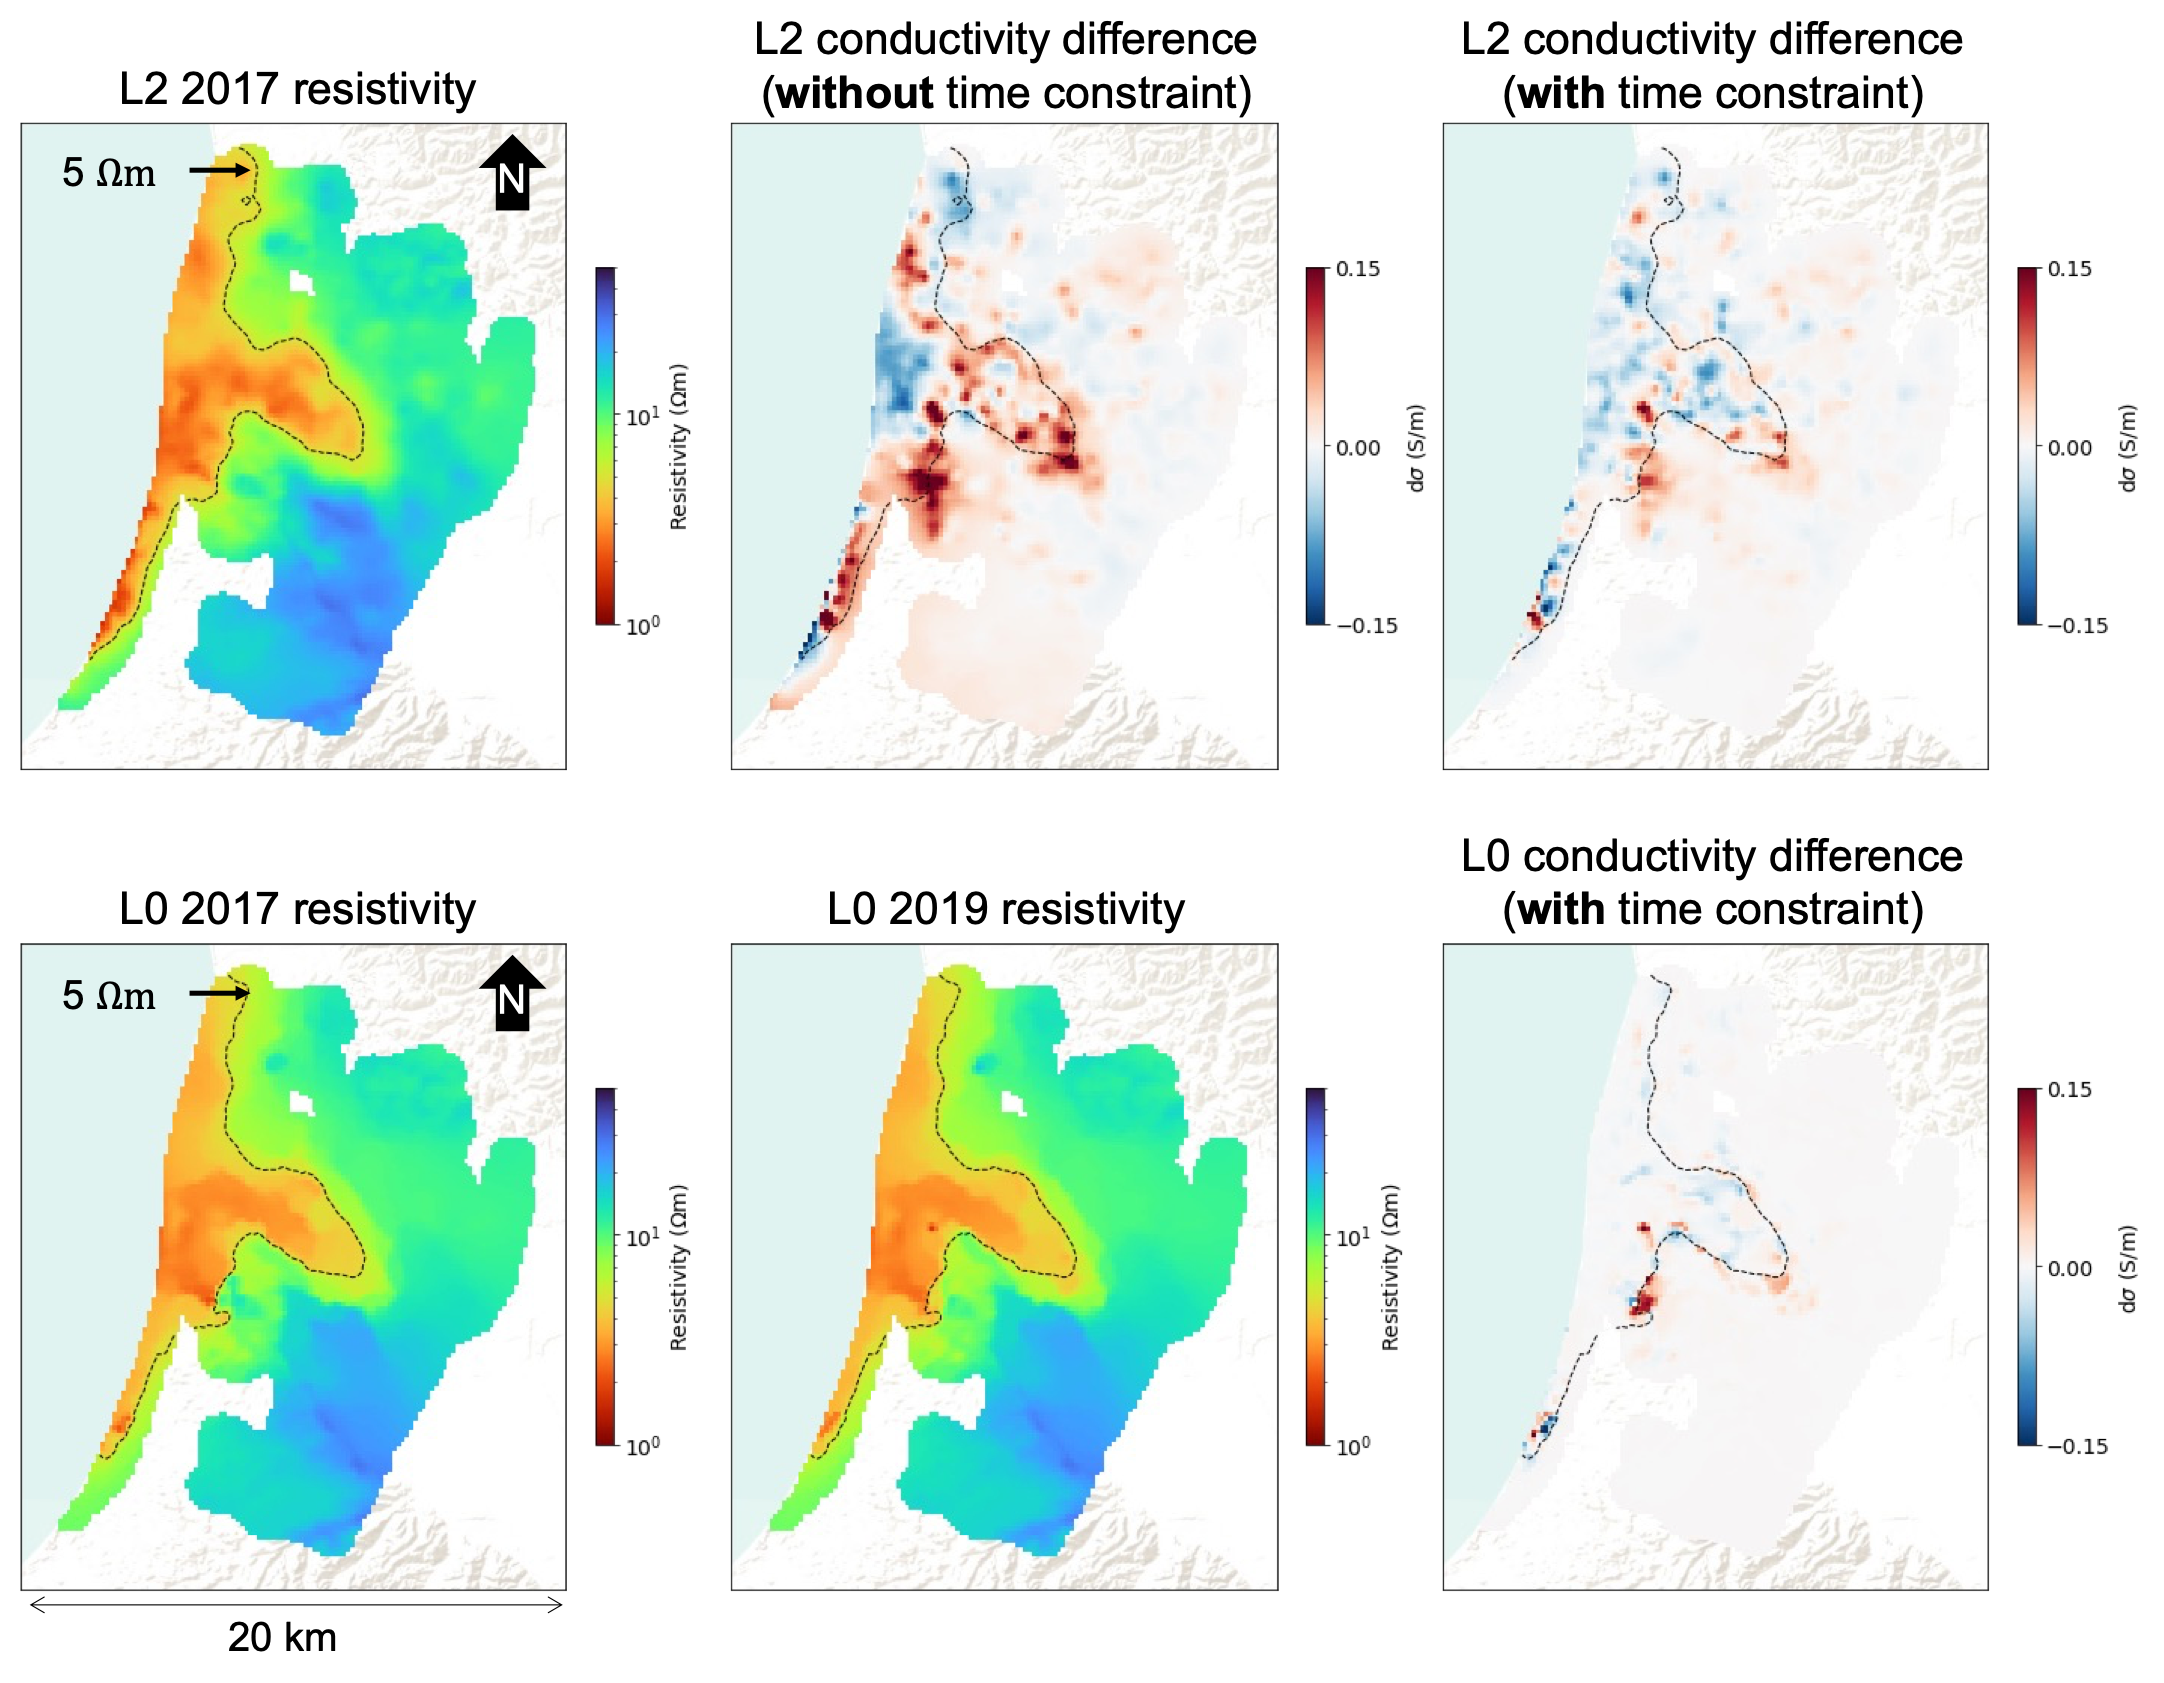
\includegraphics[width=1\textwidth]{figures/time_lapse_resistivity.png}
    \end{center}
\caption{
    Depth slices through inversion results of airborne time-domain electromagnetic data to assess seawater intrusion in California \citep{kang_time-lapse_2022}. The top row shows $\ell_2$ inversion results. The bottom row shows inversion results that make use of sparse and compact norms for both the spatial regularization and the time constraint.The black line on each image is a 5 Ohm-m-contour indicating a potential interface between saltwater and freshwater.
}
\label{fig:sparse-compact-norms-aem}
\end{figure}
